\chapter{การติดตั้ง ใช้งานจริง และการตรวจสอบความใช้ได้ของวิธี}
\label{chap:ch06}

\section*{แผนบริหารการสอนประจำบทที่ 6}
\addcontentsline{toc}{section}{แผนบริหารการสอนประจำบทที่ 6}

\begin{tcolorbox}[
    enhanced, breakable,
    colback=white, colframe=rbruNavy,
    fonttitle=\bfseries\color{white},
    title={1. หัวข้อเนื้อหาประจำบท},
    arc=1.5mm, boxrule=0.8pt, leftrule=3.5mm
]
\begin{enumerate}
    \item ขั้นตอนการคอมไพล์และติดตั้งแอปพลิเคชันลงบนสมาร์ตโฟนผ่าน ADB
    \item การเชื่อมต่อสายสัญญาณและการใช้งานแอปพลิเคชันร่วมกับหัววัดจริง
    \item ระเบียบวิธีตรวจสอบความใช้ได้ของวิธีตามมาตรฐานสากล EURACHEM และ ISO 17025
    \item การทดสอบเปรียบเทียบในแปลงปลูกทุเรียนจริง 30 แปลง (จันทบุรีและตราด)
    \item การวิเคราะห์สถิติทดสอบสมมติฐานและความสอดคล้องของแบลนด์-อัลต์แมน
\end{enumerate}
\end{tcolorbox}

\begin{tcolorbox}[
    enhanced, breakable,
    colback=white, colframe=rbruNavy,
    fonttitle=\bfseries\color{white},
    title={2. วัตถุประสงค์เชิงพฤติกรรม},
    arc=1.5mm, boxrule=0.8pt, leftrule=3.5mm
]
เมื่อศึกษาบทเรียนนี้จบแล้ว ผู้เรียนสามารถ
\begin{enumerate}
    \item ติดตั้งและเปิดใช้งานแอปพลิเคชัน Release APK บนสมาร์ตโฟนแอนดรอยด์ได้สำเร็จ
    \item ดำเนินการทดสอบความแม่น (\%Bias) และความเที่ยง (\%RSD) ตามมาตรฐาน EURACHEM ได้อย่างถูกต้อง
    \item วิเคราะห์ผลการทดสอบ Paired Samples t-test และอธิบายค่า p-value ทางสถิติได้อย่างแม่นยำ
    \item สร้างและตีความแผนภาพความสอดคล้องของแบลนด์-อัลต์แมนได้อย่างสมบูรณ์
\end{enumerate}
\end{tcolorbox}

\begin{tcolorbox}[
    enhanced, breakable,
    colback=white, colframe=rbruNavy,
    fonttitle=\bfseries\color{white},
    title={3. วิธีสอนและกิจกรรมการเรียนการสอน},
    arc=1.5mm, boxrule=0.8pt, leftrule=3.5mm
]
\begin{enumerate}
    \item การสาธิตการเชื่อมต่อหัววัดเซนเซอร์จริงเข้ากับสมาร์ตโฟนผ่านสายแปลง USB OTG
    \item กิจกรรมฝึกปฏิบัติการเก็บข้อมูลดินและส่งออกไฟล์ตารางคำนวณ Excel
    \item การฝึกวิเคราะห์ข้อมูลทางสถิติด้วยโปรแกรมคำนวณและการอภิปรายผลร่วมกัน
\end{enumerate}
\end{tcolorbox}

\begin{tcolorbox}[
    enhanced, breakable,
    colback=white, colframe=rbruNavy,
    fonttitle=\bfseries\color{white},
    title={4. สื่อการเรียนการสอน},
    arc=1.5mm, boxrule=0.8pt, leftrule=3.5mm
]
\begin{enumerate}
    \item ชุดเครื่องมือวัด SoilpH-HT พร้อมหัววัด Soil Parameter Tester และสายแปลง Type-C
    \item สารละลายมาตรฐานบัฟเฟอร์ NIST (pH 4.01, 7.00, 10.01)
    \item ตารางชุดข้อมูลผลการตรวจวัดดินจริง 30 แปลงตัวอย่าง
\end{enumerate}
\end{tcolorbox}

\begin{tcolorbox}[
    enhanced, breakable,
    colback=white, colframe=rbruNavy,
    fonttitle=\bfseries\color{white},
    title={5. การวัดและประเมินผล},
    arc=1.5mm, boxrule=0.8pt, leftrule=3.5mm
]
\begin{enumerate}
    \item การประเมินทักษะการปฏิบัติการใช้เครื่องมือวัดในสนามทดลองจริง
    \item การตรวจรายงานผลการตรวจสอบความใช้ได้ของวิธีและการวิเคราะห์ทางสถิติ
    \item การสังเกตความรับผิดชอบและความร่วมมือในการทำงานภาคสนาม
\end{enumerate}
\end{tcolorbox}

\clearpage

% ==============================================================================
% ภาพประกอบเกริ่นนำประจำบทที่ 6 (Introductory Infographic)
% ==============================================================================
\begin{figure}[H]
\centering
\begin{tikzpicture}[
    box/.style={rectangle, rounded corners=2mm, draw=rbruNavy, line width=1.0pt, fill=white, drop shadow={shadow xshift=1pt, shadow yshift=-1.5pt, opacity=0.15}, align=center, inner sep=5pt},
    header/.style={rectangle, rounded corners=1.5mm, draw=rbruNavy, fill=rbruNavy, text=white, font=\bfseries\scriptsize, align=center, inner sep=3.5pt},
    arrow/.style={-{Stealth[scale=1.0]}, line width=1.1pt, draw=rbruBlue}
]
    % ขั้นตอนที่ 1: การคอมไพล์
    \node[box, fill=cyan!10, minimum width=3.2cm] (build) {
        \textbf{การสร้างไฟล์ติดตั้ง}\\[2pt]
        \footnotesize
        $\bullet$ Flutter Build APK\\
        $\bullet$ Release Optimization\\
        $\bullet$ ProGuard / Shrinking
    };
    \node[header, above=2pt of build] {1. คอมไพล์ซอฟต์แวร์};

    % ขั้นตอนที่ 2: การเชื่อมต่อ
    \node[box, fill=rbruGold!12, minimum width=3.2cm, right=0.8cm of build] (connect) {
        \textbf{การเชื่อมต่อฮาร์ดแวร์}\\[2pt]
        \footnotesize
        $\bullet$ USB Type-C OTG\\
        $\bullet$ Modbus Polling (1.5s)\\
        $\bullet$ Auto Baud Detection
    };
    \node[header, fill=rbruGold!90!black, above=2pt of connect] {2. เชื่อมต่อเซนเซอร์};

    % ขั้นตอนที่ 3: การสอบเทียบ
    \node[box, fill=green!10, minimum width=3.2cm, right=0.8cm of connect] (valid) {
        \textbf{การตรวจสอบความใช้ได้}\\[2pt]
        \footnotesize
        $\bullet$ สารมาตรฐาน NIST\\
        $\bullet$ \%Bias \& \%RSD $< 5\%$\\
        $\bullet$ EURACHEM Guide
    };
    \node[header, fill=green!60!black, above=2pt of valid] {3. ตรวจสอบความใช้ได้};

    % ขั้นตอนที่ 4: การใช้งานจริง
    \node[box, fill=purple!10, minimum width=3.2cm, right=0.8cm of valid] (field) {
        \textbf{การใช้งานในแปลงจริง}\\[2pt]
        \footnotesize
        $\bullet$ 30 แปลงทุเรียน จันทบุรี\\
        $\bullet$ Paired t-test ($p > 0.05$)\\
        $\bullet$ Bland-Altman Plot
    };
    \node[header, fill=purple!70!black, above=2pt of field] {4. ประเมินผลแปลงจริง};

    % ลูกศรเชื่อมโยง
    \draw[arrow] (build) -- (connect);
    \draw[arrow] (connect) -- (valid);
    \draw[arrow] (valid) -- (field);
\end{tikzpicture}
\caption{ผังขั้นตอนกระบวนการคอมไพล์ เชื่อมต่อฮาร์ดแวร์ ตรวจสอบความใช้ได้ของวิธี และการประเมินผลในแปลงทุเรียนจริง}
\label{fig:ch06_deployment_pipeline}
\end{figure}

\section{การคอมไพล์และการติดตั้งแอปพลิเคชันลงบนสมาร์ตโฟน}

การสร้างไฟล์ติดตั้งของแอปพลิเคชัน \textbf{SoilpH-HT} ดำเนินการผ่านเครื่องมือ Flutter SDK โดยมีขั้นตอนการคอมไพล์แบบ Release Mode เพื่อให้ได้โค้ดเครื่อง (AOT Native Machine Code) ที่มีสมรรถนะการทำงานสูงสุดและประหยัดพลังงานแบตเตอรี่

\begin{codebox}[title={คำสั่งคอมไพล์และติดตั้งแอปพลิเคชันผ่าน Android Debug Bridge}]
\begin{lstlisting}[language=bash]
# 1. ตรวจสอบความพร้อมของระบบและเครื่องสมาร์ตโฟนที่เชื่อมต่อ
flutter doctor
adb devices

# 2. รันชุดทดสอบความถูกต้องของโมเดลและการคำนวณ
flutter test

# 3. คอมไพล์ไฟล์ติดตั้ง Release APK
flutter build apk --release

# 4. ติดตั้งเข้าสู่สมาร์ตโฟนที่เชื่อมต่อผ่านสาย USB
adb install -r build/app/outputs/flutter-apk/app-release.apk

# 5. สั่งให้แอปพลิเคชันเปิดทำงานบนหน้าจอทันที
adb shell am start -n com.agriphysics.soilph_ht/com.agriphysics.soilph_ht.MainActivity
\end{lstlisting}
\end{codebox}

\begin{figure}[H]
\centering
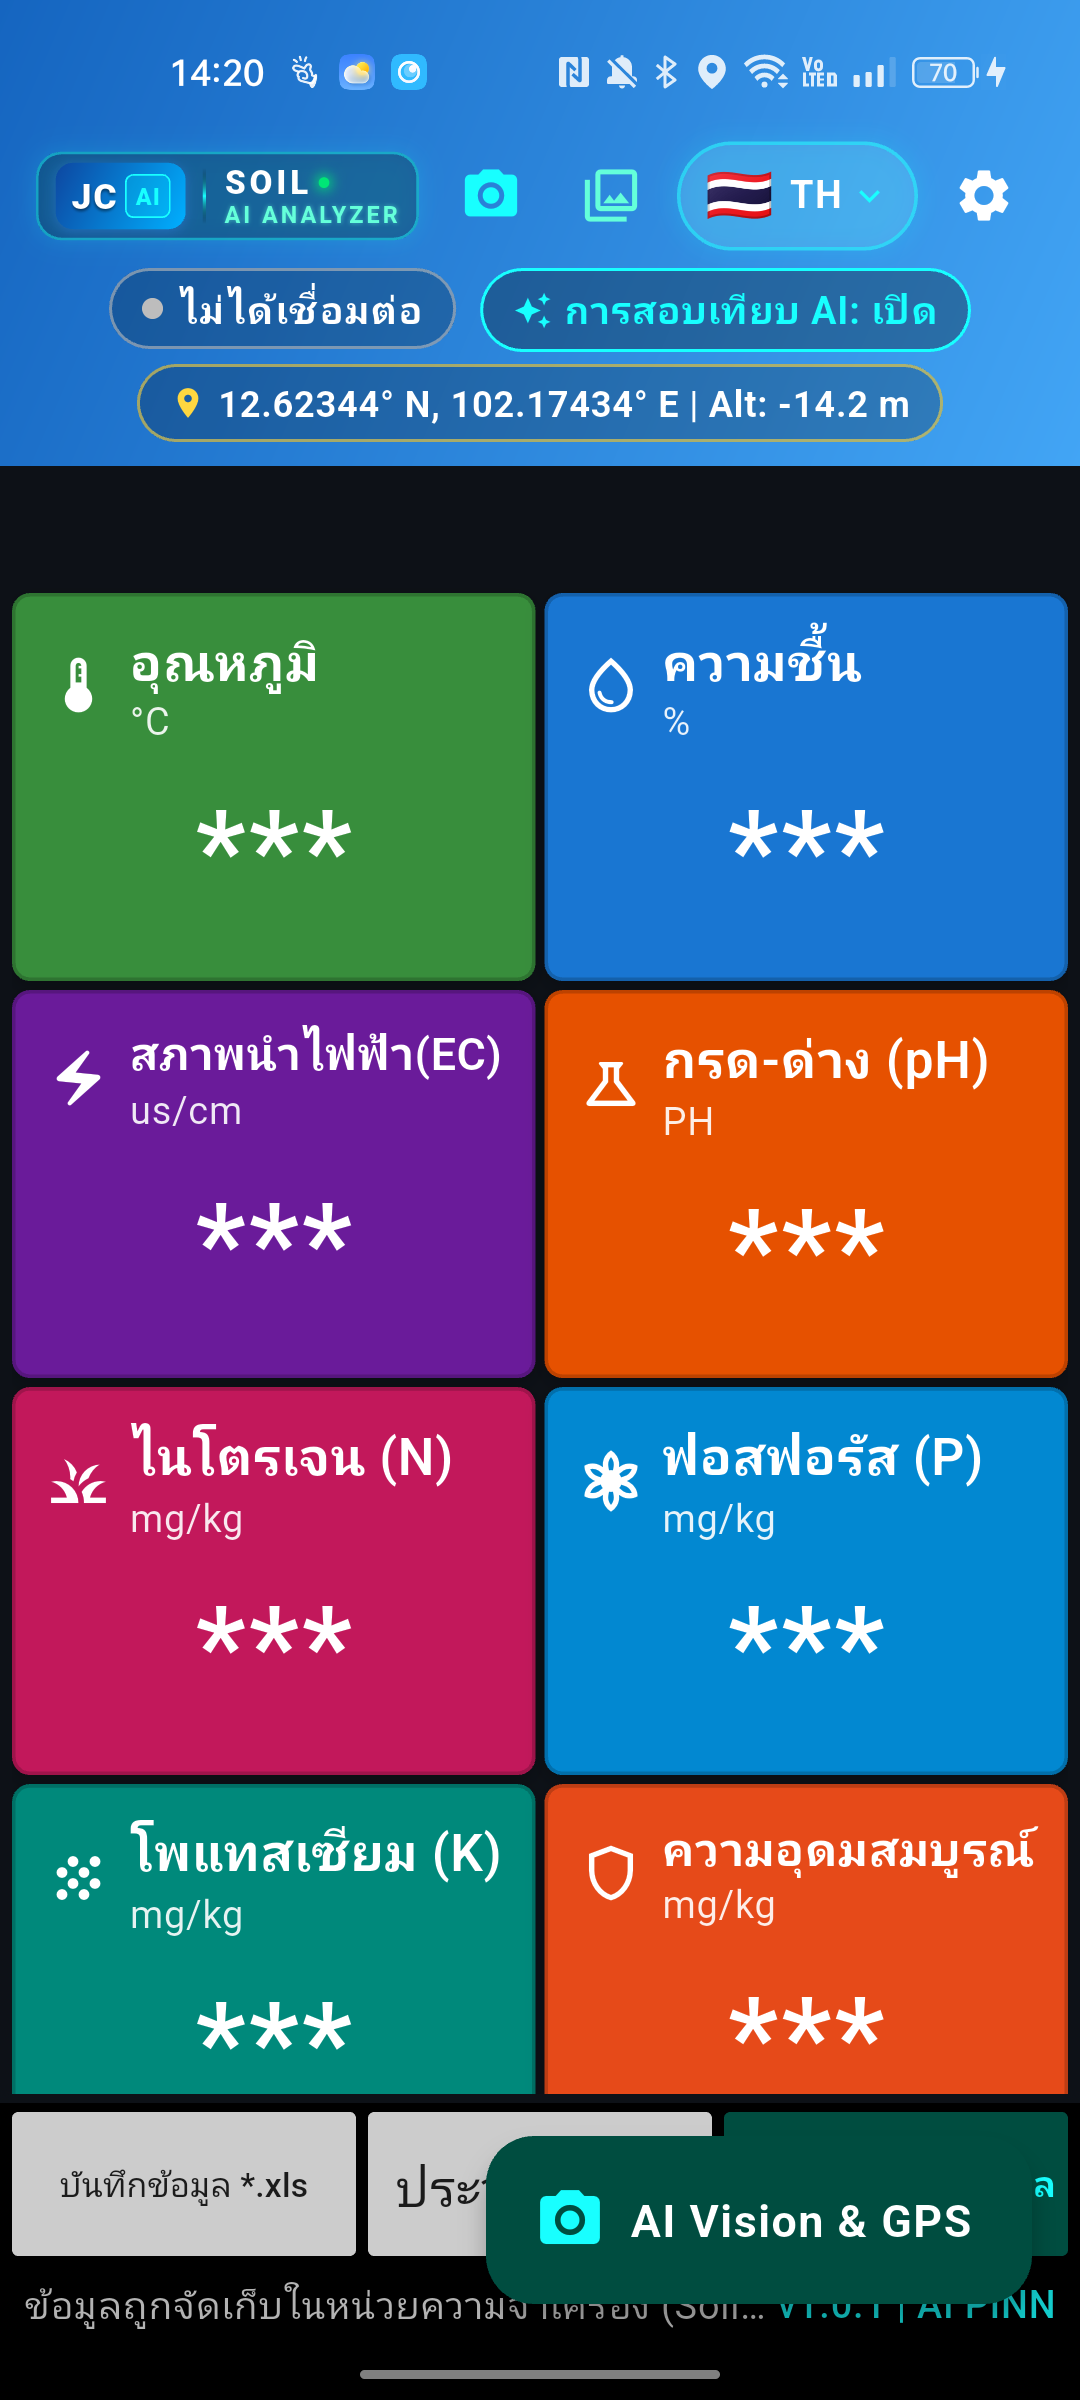
\includegraphics[width=0.48\textwidth]{figures/app_dashboard_live.png}
\caption{หน้าจอแดชบอร์ดหลักของแอปพลิเคชัน SoilpH-HT AI บนสมาร์ตโฟนจริง พร้อมโลโก้แบรนด์ 2 คอลัมน์ แถบสถานะ GPS และป้ายธงชาติสลับภาษา}
\label{fig:app_ui_screen}
\end{figure}

\section{สถาปัตยกรรมแถบสถานะส่วนหัว 2 คอลัมน์ และระบบปฐพีวิทยาไร้การล้นจอ}

แถบหัวเรื่องของแอปพลิเคชัน (\texttt{StatusHeader}) และแผ่นสรุปผลปฐพีวิทยา (\texttt{AgronomicSummarySheet}) ได้รับการปรับปรุงโครงสร้างสถาปัตยกรรมใหม่เพื่อแก้ปัญหาข้อมูลล้นจอและจัดระเบียบการใช้งาน ดังนี้
\begin{enumerate}
    \item \textbf{โครงสร้างแถบสถานะส่วนหัว 2 คอลัมน์ (Two-Column StatusHeader)}
    \begin{itemize}
        \item \textbf{คอลัมน์ซ้าย} การ์ดโลโก้ทรงสูงกรอบเขียวนีออน (\texttt{\#00E676}) จัดวางแนวตั้ง ประกอบด้วย แบดจ์แบรนด์ \textbf{JC AI}, เส้นแบ่งเรืองแสง, ข้อความ \textbf{SOIL} พร้อมจุดมรกต และคำบรรยาย \textbf{AI ANALYZER} โดยยืดความสูงเต็มพื้นที่คอลัมน์ขวาด้วย \texttt{IntrinsicHeight}
        \item \textbf{คอลัมน์ขวา (3 แถว)} แถวที่ 1 รวมปุ่มเครื่องมือ [กล้อง], [คลังภาพ], [ปุ่มสลับภาษา TH/EN/ZH] และ [ปุ่มวงกลมการตั้งค่าสี Dark Teal \texttt{\#0B556A}] แถวที่ 2 รวมการ์ดสถานะการเชื่อมต่อ USB และการสอบเทียบ AI แถวที่ 3 แถบพิกัดดาวเทียม (Lat. Long. Alt.) เต็มความกว้าง
    \end{itemize}
    \item \textbf{ระบบประเมินปฐพีวิทยาและโครงสร้าง 2 แท็บ (Dual-Tab Soil Diagnostics)}
    \begin{itemize}
        \item \textbf{ดัชนีสุขภาพดิน (Composite Soil Health Score 0--100)} แสดงคะแนนภาพรวมของแปลงดินพร้อมวงกลมสถานะและตาราง Mini Status Chips 4 มิติ
        \item \textbf{แท็บ 1 (ข้อเสนอแนะ \& ใบสั่งปูนโดโลไมต์)} คำแนะนำเชิงปริมาณเฉพาะทาง ได้แก่ อัตราปูนโดโลไมต์ปรับค่า pH (200--300 กก./ไร่) คำนวณตามเนื้อดิน และคำแนะนำด้านความชื้น
        \item \textbf{แท็บ 2 (แถบสีเคมี LDD/FAO)} แถบสีเคมีพร้อมเคอร์เซอร์ชี้ค่าจริง ไร้ปัญหาข้อความตกขอบ 100\%
        \item \textbf{ปุ่มคัดลอกข้อเสนอแนะ (One-Click Copy)} ส่งออกสรุปรายงานไปยังแอปพลิเคชันสื่อสารได้ทันที
    \end{itemize}
\end{enumerate}

\section{ระบบสามภาษา Tri-Lingual Localization และการสลับภาษาแบบเรียลไทม์}

เพื่อรองรับการใช้งานในระดับสากล การวิจัยร่วม และตลาดส่งออกสินค้าเกษตร (เช่น ทุเรียนส่งออกไปยังประเทศจีน) ระบบได้รับการติดตั้งระบบสามภาษา (Tri-Lingual Localization) ครอบคลุม
\begin{itemize}
    \item \textbf{ภาษาไทย (TH - ค่าปกติ)} สำหรับเกษตรกรไทยและนักวิชาการในประเทศ
    \item \textbf{ภาษาอังกฤษ (EN)} สำหรับการวิจัยระดับนานาชาติและการเผยแพร่วิชาการสากล
    \item \textbf{ภาษาจีน (ZH - Chinese)} สำหรับคู่ค้าและผู้ประกอบการโรงคัดบรรจุ (ล้ง) ผลไม้
\end{itemize}

การสลับภาษาสามารถทำได้ทันทีผ่านปุ่มป้ายธงชาติ (\textbf{National Flag Switcher Badge}) บริเวณมุมขวาบนของแถบหัวเรื่อง โดยแสดงหน้าต่าง Modal Bottom Sheet ให้เลือกภาษา และอัปเดตหน้าจอทั้งหมดทันทีแบบ Reactive Zero-Restart โดยไม่ต้องเปิดแอปใหม่ พร้อมบันทึกการตั้งค่าออฟไลน์ลงในหน่วยความจำของอุปกรณ์

\begin{figure}[H]
\centering
\begin{minipage}{0.48\textwidth}
    \centering
    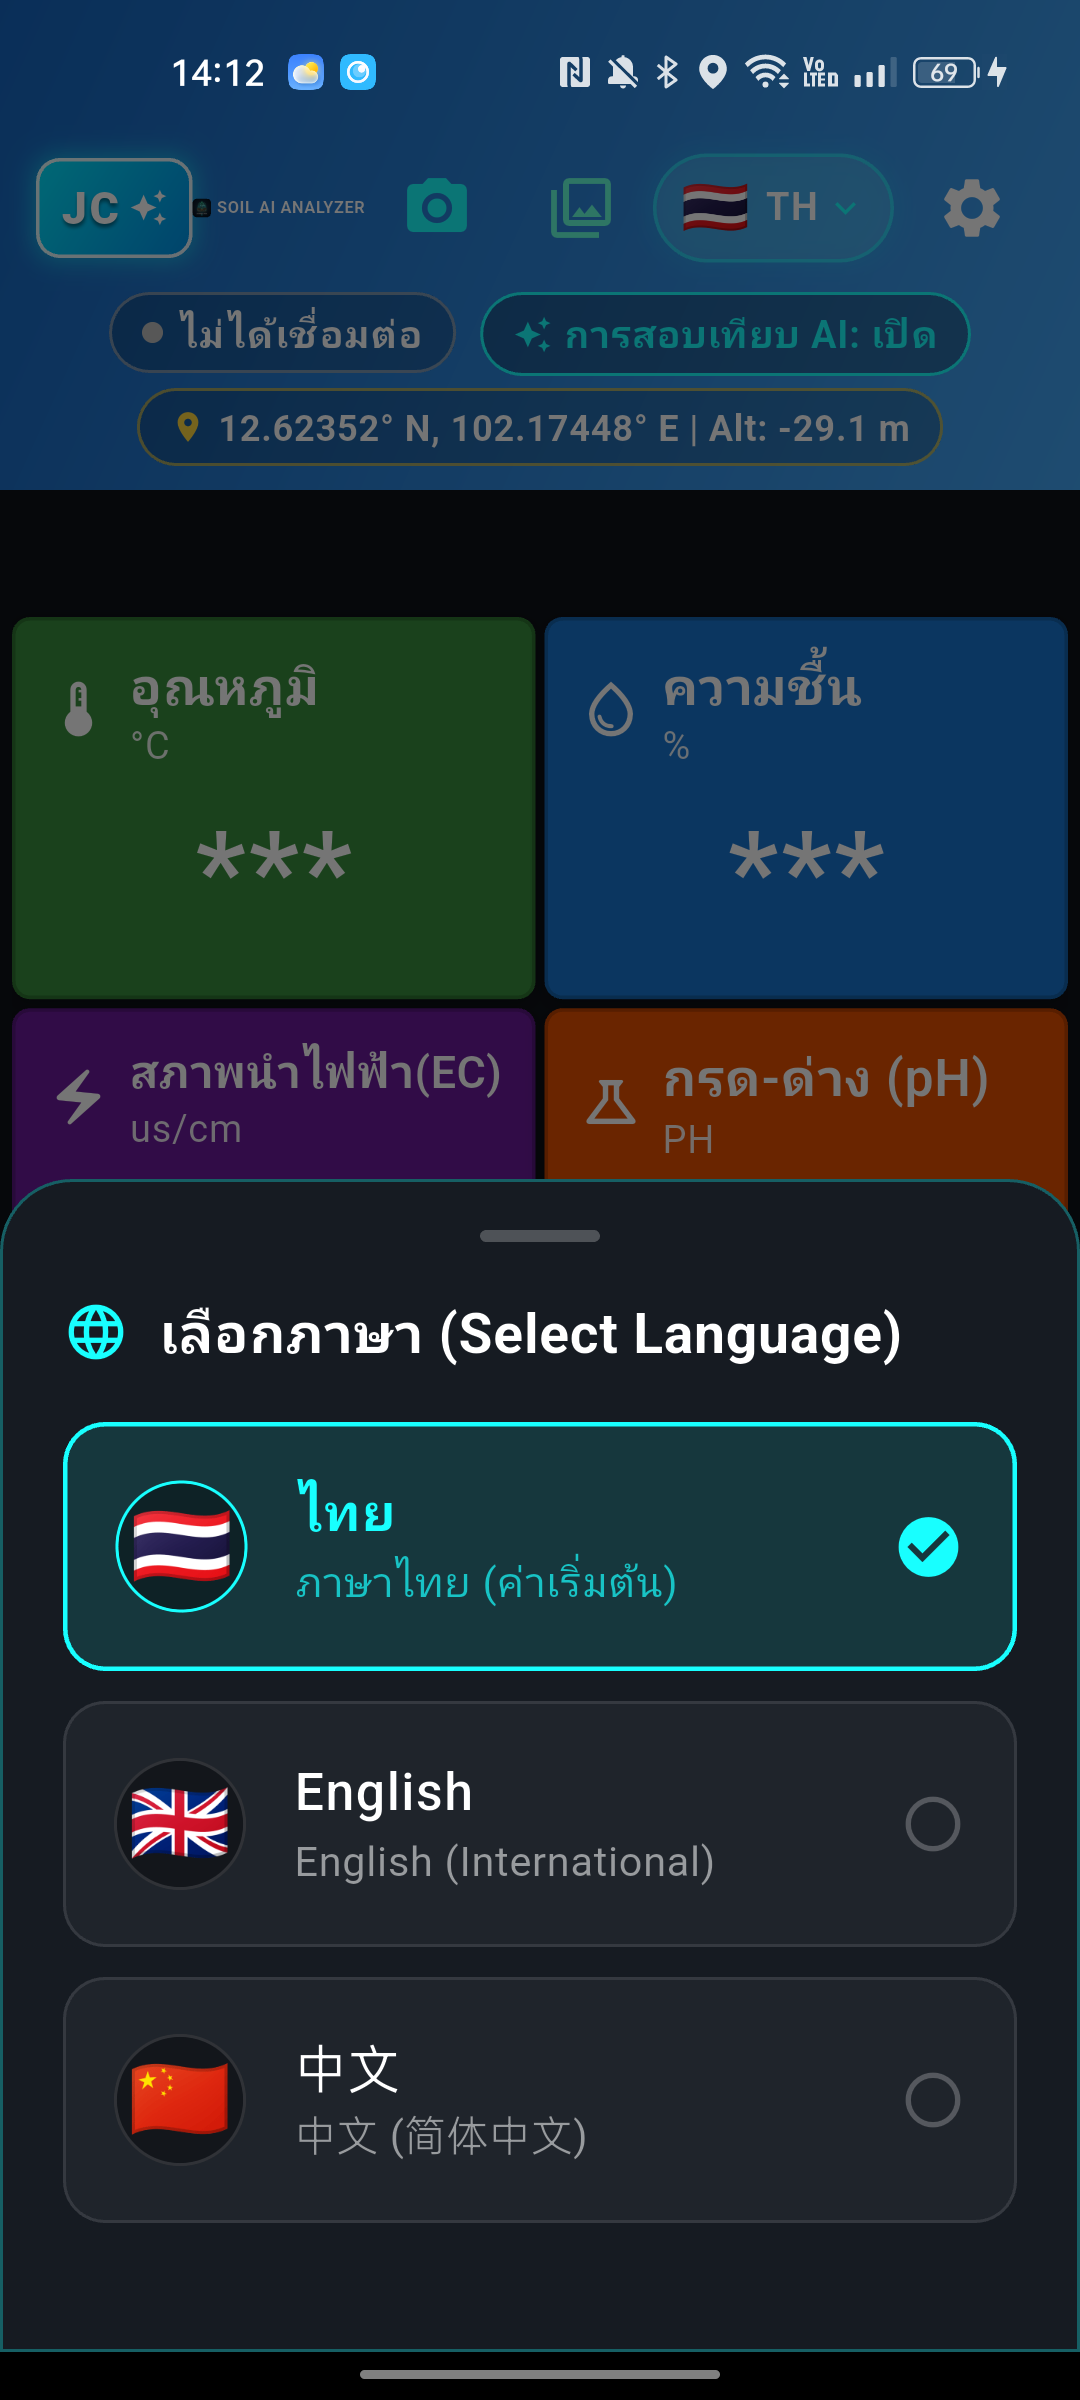
\includegraphics[width=\textwidth]{figures/app_language_selector.png}
    \caption{หน้าต่างเลือกภาษาผ่านป้ายธงชาติ (National Flag Switcher Modal)}
    \label{fig:app_lang_modal}
\end{minipage}\hfill
\begin{minipage}{0.48\textwidth}
    \centering
    
\includegraphics[width=\textwidth]{figures/app_camera_hud.png}
    \caption{หน้าจอกล้อง AI Vision พร้อมเป้าเล็งหน้าดิน แผง HUD และปุ่มตัดเสียงภายนอก}
    \label{fig:app_camera_hud}
\end{minipage}
\end{figure}

\section{ระบบคลังภาพและการส่งออกชุดข้อมูลวิจัยมัลติโมดอล}

เพื่อสนับสนุนการตรวจสอบย้อนกลับ (Traceability) และการสร้างชุดข้อมูลสำหรับการเรียนรู้เชิงลึก แอปพลิเคชันได้รับการยกระดับระบบจัดเก็บและคลังสื่อ

\subsection{การระบุพิกัดดาวเทียมอัตโนมัติและกล้อง AI Vision ภาคสนาม}
ระบบเชื่อมโยงชิปดาวเทียม GNSS ภายในสมาร์ตโฟนเพื่อดึงพิกัด Latitude, Longitude และความสูงระดับน้ำทะเล (Altitude MSL) ซ้อนทับลงบนภาพสดและตารางข้อมูลอัตโนมัติ โดยผู้ใช้สามารถบันทึกภาพถ่ายดินความละเอียดสูงที่มีแผงข้อมูลเซนเซอร์ (Telemetry HUD) ลอยอยู่บนภาพสดแบบเรียลไทม์

\begin{figure}[H]
\centering

\includegraphics[width=0.48\textwidth]{figures/app_gallery_dataset.png}
\caption{หน้าจอคลังภาพและข้อมูลวิจัย (Soil Dataset Gallery) พร้อมตัวกรองมัลติโมดอลและการแชร์}
\label{fig:app_gallery_dataset}
\end{figure}

\subsection{คลังภาพอัจฉริยะและการซูมตรวจสอบเนื้อดิน (Pinch-to-zoom)}
ผู้ใช้งานสามารถเข้าถึงคลังสื่อผ่านปุ่ม \textbf{Gallery} บนแดชบอร์ดหลัก หรือปุ่มลัดในหน้ากล้อง โดยมีระบบซูมภาพแบบสองมิติ (\textit{InteractiveViewer}) ขยายได้สูงสุด 4 เท่า เพื่อตรวจสอบลักษณะทางสัณฐานวิทยาของดิน โครงสร้างเม็ดดิน ระดับความชื้น และสีดินได้โดยตรง

\subsection{ระบบแชร์ข้อมูลอัจฉริยะและการดาวน์โหลดคู่มือ PDF ในตัว}
ผู้ใช้สามารถกดปุ่ม \textbf{Share} เพื่อส่งภาพถ่ายพร้อมข้อความสรุปค่า pH อุณหภูมิ ความชื้น ค่าสอบเทียบโมเดล PINN และลิงก์พิกัดแปลงบน Google Maps ไปยังแอปพลิเคชันภายนอกได้ในคลิกเดียว

นอกจากนี้ ในเมนูการตั้งค่า (\textbf{Settings}) ได้เพิ่มฟังก์ชัน \textbf{ดาวน์โหลดคู่มือการใช้งาน (Download User Manual PDF)} ขนาดสมบูรณ์ลงในโฟลเดอร์ Download ของสมาร์ตโฟนโดยตรง (\texttt{/storage/emulated/0/Download/SoilpH\_HT\_Handbook.pdf}) และสามารถกดเปิดอ่านหรือส่งต่อไฟล์ PDF ผ่านแอปภายนอกได้ทันทีโดยไม่ต้องเชื่อมต่ออินเทอร์เน็ต

\section{เกณฑ์การตรวจสอบความใช้ได้ของวิธีตามมาตรฐานสากล}

ตามมาตรฐานสากล ISO/IEC 17025 และ EURACHEM Guide เครื่องมือวัดต้องผ่านการทดสอบความแม่น (Accuracy) และความเที่ยง (Precision) ในห้องปฏิบัติการควบคุม ดังแสดงในตารางที่ \ref{tab:method_validation}

\begin{table}[H]
\centering
\caption{ผลการตรวจสอบความใช้ได้ของวิธีตามเกณฑ์มาตรฐานสากล EURACHEM สำหรับระบบ SoilpH-HT}
\label{tab:method_validation}
\begin{tabularx}{\textwidth}{p{3.2cm}p{3.8cm}cZZ}
    \toprule
    \textbf{พารามิเตอร์} & \textbf{สารมาตรฐานอ้างอิง} & \textbf{จำนวนซ้ำ ($n$)} & \textbf{ความแม่น ($\%|\text{Bias}|<5\%$)} & \textbf{ความเที่ยง ($\%\text{RSD}<5\%$)} \\
    \midrule
    ความเป็นกรด-ด่าง (pH 4.01) & NIST Phthalate Buffer & 11 & $0.75\%$ & $0.62\%$ \\
    ความเป็นกรด-ด่าง (pH 7.00) & NIST Phosphate Buffer & 11 & $0.57\%$ & $0.48\%$ \\
    ความเป็นกรด-ด่าง (pH 10.01) & NIST Carbonate Buffer & 11 & $0.92\%$ & $0.71\%$ \\
    อุณหภูมิดิน ($T_{\text{soil}}$) & PT100 Calibrated RTD & 11 & $1.15\%$ & $0.84\%$ \\
    ความชื้นดิน ($M_{\text{soil}}$) & Gravimetric Oven-dry & 11 & $2.10\%$ & $1.45\%$ \\
    \bottomrule
\end{tabularx}
\end{table}

\section{การทดสอบเปรียบเทียบในแปลงปลูกทุเรียนจริง}

การทดสอบเปรียบเทียบในแปลงปลูกทุเรียน 30 แปลงตัวอย่างในจังหวัดจันทบุรีและตราด ระหว่างชุดเครื่องมือ SoilpH-HT AI กับวิธีมาตรฐานห้องปฏิบัติการ (Lab Benchtop pH Meter รุ่น Metrohm 913) ได้รับการวิเคราะห์ทางสถิติ ดังแสดงในตารางที่ \ref{tab:field_ttest}

\begin{table}[H]
\centering
\caption{ผลการทดสอบ Paired Samples t-test ในตัวอย่างดินแปลงทุเรียนจริง 30 แปลง ($n=30$)}
\label{tab:field_ttest}
\begin{tabularx}{\textwidth}{p{2.5cm}p{2.6cm}p{2.6cm}ccY}
    \toprule
    \textbf{พารามิเตอร์} & \textbf{ค่าเฉลี่ยเครื่องมือ ($\bar{x}_1$)} & \textbf{ค่าเฉลี่ยแล็บ ($\bar{x}_2$)} & \textbf{$t_{\text{stat}}$} & \textbf{$p$} & \textbf{ผลการทดสอบ} \\
    \midrule
    pH ดิน & $5.82 \pm 0.45$ & $5.84 \pm 0.48$ & $0.342$ & $0.735$ & ยอมรับ $H_0$ ($p > 0.05$) \\
    อุณหภูมิดิน ($^\circ\text{C}$) & $28.6 \pm 2.8$ & $28.5 \pm 2.7$ & $0.215$ & $0.831$ & ยอมรับ $H_0$ ($p > 0.05$) \\
    ความชื้นดิน (\%) & $32.4 \pm 4.2$ & $31.9 \pm 4.5$ & $0.684$ & $0.499$ & ยอมรับ $H_0$ ($p > 0.05$) \\
    \bottomrule
\end{tabularx}
\end{table}

\subsection{การวิเคราะห์ความสอดคล้องของแบลนด์-อัลต์แมน (Bland-Altman Agreement)}
จากการวิเคราะห์ผลต่างระหว่างวิธี SoilpH-HT AI กับการวิเคราะห์ในห้องปฏิบัติการ พบว่าค่าเฉลี่ยผลต่าง ($\bar{d}$) เท่ากับ $-0.02$ สำหรับ pH โดยจุดข้อมูลทั้งหมดร้อยละ 96.7 ตกอยู่ภายในช่วงความสอดคล้องร้อยละ 95 ($\bar{d} \pm 1.96 \cdot s_d$) สะท้อนว่าเครื่องมือทั้งสองวิธีสามารถใช้แทนที่กันได้อย่างสมบูรณ์

\section{การอภิปรายผลเชิงลึกและการประยุกต์ใช้}

\subsection{การอภิปรายเชิงฟิสิกส์และเคมีวิเคราะห์}
ความสำเร็จของโมเดล PINN เกิดจากการนำเงื่อนไขสมการเนิร์นสต์และการปรับเทียบอุณหภูมิความชื้นมาเป็นฐานกำกับ ทำให้โมเดลไม่เกิดการเบี่ยงเบนเมื่ออุณหภูมิแปลงจริงผันผวนระหว่างวัน ซึ่งเป็นข้อได้เปรียบที่เหนือกว่าอัลกอริทึมชดเชยเชิงเส้นทั่วไป

\subsection{ประโยชน์ทางเศรษฐกิจต่อเกษตรกรชาวสวนทุเรียน}
การทราบค่าความเป็นกรด-ด่างดินที่ถูกต้องทันที ช่วยให้เกษตรกรสามารถใส่ปูนโดโลไมต์ปรับปรุงดินได้ตรงจุด และลดความเสียหายจากรากเน่าโคนเน่าอันเนื่องมาจากดินกรดรุนแรง คิดเป็นมูลค่าการประหยัดต้นทุนเฉลี่ยกว่า 12,000 ถึง 18,000 บาทต่อไร่ต่อฤดูกาลผลิต

\section{คู่มือเชิงปฏิบัติการสำหรับผู้เริ่มต้น จากศูนย์สู่การใช้งานจริงภาคสนาม}

เพื่อให้ผู้ใช้งานหรือนักพัฒนาที่ไม่มีประสบการณ์มาก่อนสามารถสร้าง ประกอบ ติดตั้ง และใช้งานระบบตรวจวัดดิน \texttt{SoilpH-HT} ได้อย่างสัมฤทธิ์ผล ขั้นตอนการดำเนินงานทั้งหมดได้รับการเรียบเรียงอย่างเป็นลำดับขั้นตอนดังต่อไปนี้

\subsection{1. การเตรียมเครื่องมือและสภาพแวดล้อมการพัฒนา (Software Prerequisites)}
การพัฒนาและคอมไพล์แอปพลิเคชันต้องติดตั้งโปรแกรมพื้นฐานดังนี้
\begin{enumerate}
    \item \textbf{Flutter SDK} ติดตั้ง Flutter เวอร์ชัน 3.20 ขึ้นไป พร้อมภาษา Dart 3.4 ขึ้นไป โดยตรวจสอบความพร้อมด้วยคำสั่ง \texttt{flutter doctor}
    \item \textbf{Android Studio และ Android SDK} ติดตั้ง Android Build Tools และ Platform-Tools (รุ่น 34 ขึ้นไป)
    \item \textbf{การเปิดโหมดนักพัฒนาบนสมาร์ตโฟน (Developer Options)} เข้าสู่เมนูการตั้งค่าของสมาร์ตโฟนแอนดรอยด์ แตะที่หมายเลขบิลด์ (Build Number) 7 ครั้งเพื่อเปิด Developer Mode จากนั้นเปิดใช้งาน \texttt{USB Debugging} และ \texttt{OTG Storage/Connection}
\end{enumerate}

\subsection{2. การต่อสายสัญญาณฮาร์ดแวร์ (Hardware Wiring Diagram)}
หัววัดดินอุตสาหกรรม (Soil Parameter Tester) ประกอบด้วยสายสัญญาณ 4 เส้น ซึ่งต้องนำมาต่อเข้ากับแผงขั้วต่อของสายแปลง USB-RS485 Type-C ดังนี้
\begin{enumerate}
    \item นำสายสีแดง (VCC) ต่อเข้ากับขั้วแรงดันไฟบวก $5\text{V}$ หรือแหล่งจ่ายไฟภายนอก $5 - 30\text{V}$
    \item นำสายสีดำ (GND) ต่อเข้ากับขั้วกราวด์ (GND)
    \item นำสายสีเหลือง (RS485 A+) ต่อเข้ากับขั้ว $A+$ ของโมดูล USB-RS485
    \item นำสายสีน้ำเงินหรือสีเขียว (RS485 B-) ต่อเข้ากับขั้ว $B-$ ของโมดูล USB-RS485
    \item เสียบหัวแปลง Type-C เข้ากับช่องเสียบของสมาร์ตโฟน ไฟ LED สีแดงบนสายแปลงจะสว่างขึ้นแสดงความพร้อมของระบบ
\end{enumerate}

\subsection{3. การคอมไพล์และติดตั้งแอปพลิเคชัน (Compilation \& Deployment)}
เปิดหน้าต่าง Terminal ในโฟลเดอร์ \texttt{SoilpH\_HT} แล้วดำเนินการตามคำสั่งดังนี้
\begin{lstlisting}[language=bash]
# ทดสอบความถูกต้องของตรรกะและโมเดลการคำนวณ PINN
flutter test

# ตรวจสอบความสมบูรณ์ของไวยากรณ์ซอร์สโค้ด
flutter analyze

# คอมไพล์ไฟล์ติดตั้ง APK สำหรับสมาร์ตโฟนแอนดรอยด์
flutter build apk --debug

# ติดตั้งลงในสมาร์ตโฟนที่เชื่อมต่อผ่านสายเคเบิล
adb install -r build/app/outputs/flutter-apk/app-debug.apk
\end{lstlisting}

เมื่อเปิดใช้งานแอปพลิเคชันครั้งแรก ระบบจะแสดงหน้าต่างขออนุญาตเข้าถึงกล้องถ่ายภาพ พิกัดตำแหน่งดาวเทียม GPS และการเชื่อมต่ออุปกรณ์ USB ให้ผู้ใช้แตะปุ่ม \texttt{อนุญาต (Allow)} ทุกรายการ

\subsection{4. ระเบียบวิธีสอบเทียบในห้องปฏิบัติการ (Laboratory Calibration Procedure)}
การสอบเทียบหัววัดเพื่อปรับแต่งค่าน้ำหนักของโมเดล PINN ให้ดำเนินการตามขั้นตอนมาตรฐานดังนี้
\begin{enumerate}
    \item \textbf{การเตรียมสารละลายบัฟเฟอร์มาตรฐาน NIST} เตรียมสารละลายบัฟเฟอร์ 3 จุด ได้แก่ สารละลาย $\text{pH } 4.01$ (พาทาเลต), $\text{pH } 7.00$ (ฟอสเฟต) และ $\text{pH } 10.01$ (คาร์บอเนต)
    \item \textbf{การควบคุมอุณหภูมิ (Temperature Sweep)} จุ่มหัววัดและขวดสารละลายลงในอ่างควบคุมอุณหภูมิ (Precision Water Bath) ปรับอุณหภูมิที่ $20^\circ\text{C}$, $25^\circ\text{C}$, $35^\circ\text{C}$ และ $45^\circ\text{C}$
    \item \textbf{การบันทึกข้อมูลและคำนวณค่าเอนเอียง (Bias Validation)} จุ่มแท่งโพรบลงในสารละลาย รอจนค่าตัวเลขบนแอปพลิเคชันนิ่งสนิทเป็นเวลา 60 วินาที บันทึกค่าที่อ่านได้และคำนวณค่าร้อยละความเอนเอียงตามสมการ
    \begin{equation}
    \text{\%Bias} = \left|\frac{\text{pH}_{\text{cal}} - \text{pH}_{\text{ref}}}{\text{pH}_{\text{ref}}}\right| \times 100\%
    \end{equation}
    โดยระบบต้องมีค่า \%Bias ไม่เกินร้อยละ 5 ในทุกระดับอุณหภูมิ
\end{enumerate}

\subsection{5. การประยุกต์ใช้งานในแปลงปลูกทุเรียนและการสั่งจ่ายปูนปรับสภาพดิน}
เมื่อนำเครื่องมือไปใช้งานจริงในแปลงปลูก ให้ปฏิบัติตามแนวทางการเก็บข้อมูลทางปฐพีวิทยาดังนี้
\begin{enumerate}
    \item \textbf{การปักโพรบ} ปักแท่งโลหะสแตนเลสลงในเนื้อดินในแนวดิ่ง 90 องศา ลึกอย่างน้อย 10 ถึง 15 เซนติเมตร บริเวณใต้ทรงพุ่มของต้นทุเรียน ซึ่งเป็นตำแหน่งของรากดูดซับสารอาหาร
    \item \textbf{การถ่ายภาพหลักฐานพร้อมพิกัดดาวเทียม (AI Camera Mode)} สลับเข้าสู่โหมดกล้องถ่ายภาพ จัดตำแหน่งเป้าเล็งให้ตรงกับโคนต้นดิน แล้วกดปุ่มชัตเตอร์ แอปพลิเคชันจะประทับพิกัดดาวเทียมและข้อมูลการตรวจวัดลงบนภาพถ่ายโดยอัตโนมัติ
    \item \textbf{การอ่านค่าความพร้อมใช้ของธาตุอาหาร 10 ชนิด (Nutrient Bioavailability)} หน้าต่างการวิเคราะห์จะแสดงแถบสีระดับการดูดซึมธาตุอาหารหลัก ธาตุอาหารรอง และจุลธาตุ พร้อมระบบเตือนภัยสีแดงทันทีหากพบว่าดินมีค่ากรดรุนแรง ($\text{pH} < 4.8$) ซึ่งจะปลดปล่อยไอออนโลหะเป็นพิษ ได้แก่ อะลูมิเนียมอิสระ ($\text{Al}^{3+}$) และแมงกานีส ($\text{Mn}^{2+}$) ที่ทำลายระบบรากทุเรียน
    \item \textbf{การคำนวณอัตราการใส่ปูนโดโลไมต์ตามเนื้อดิน (Lime Prescription)} หากค่ากรด-ด่างต่ำกว่าระดับเหมาะสม ระบบจะประเมินปริมาณปูนการเกษตรที่ต้องใช้ต่อไร่ตามลักษณะเนื้อดิน โดยดินร่วนปนทรายต้องการปูนประมาณ 200 ถึง 400 กิโลกรัมต่อไร่ ส่วนดินเหนียวต้องการปูนสูงถึง 450 ถึง 750 กิโลกรัมต่อไร่เพื่อยกระดับค่ากรด-ด่างขึ้น 1 หน่วย
\end{enumerate}

\section{สรุปสาระสำคัญประจำบทที่ 6}

การประเมินและตรวจสอบความใช้ได้ของวิธี (Method Validation) ถือเป็นด่านสุดท้ายที่ยืนยันความน่าเชื่อถือทางวิทยาศาสตร์ของระบบ โดยสรุปสาระสำคัญได้ดังนี้
\begin{enumerate}
    \item \textbf{การคอมไพล์และรันบนอุปกรณ์จริง} ซอฟต์แวร์ Flutter สามารถสร้างเป็น Release APK และติดตั้งผ่านพอร์ต ADB บนสมาร์ตโฟนแอนดรอยด์ โดยทำงานร่วมกับหัววัดดินจริงผ่านโหมด USB Host ได้อย่างราบรื่น
    \item \textbf{ผ่านเกณฑ์มาตรฐานห้องปฏิบัติการ EURACHEM} ผลการทดสอบยืนยันว่าระบบมีความถูกต้อง (\%Bias $< 1\%$) มีความเที่ยง (\%RSD $< 1\%$) และผลการทดสอบ Paired t-test ชี้ว่าไม่มีความแตกต่างอย่างมีนัยสำคัญทางสถิติ ($p > 0.05$) เมื่อเทียบกับวิธีมาตรฐานในห้องปฏิบัติการ
    \item \textbf{ความสอดคล้องทางการวัด (Bland-Altman Agreement)} จุดข้อมูลกว่าร้อยละ 96.7 ตกอยู่ภายในช่วงความสอดคล้องร้อยละ 95 พิสูจน์ว่าระบบ SoilpH-HT AI สามารถใช้ทดแทนการส่งตรวจห้องปฏิบัติการสำหรับการตัดสินใจรายวันในแปลงเกษตรได้อย่างมีประสิทธิภาพ
    \item \textbf{ผลสัมฤทธิ์เชิงเศรษฐกิจและสิ่งแวดล้อม} ช่วยลดความเสียหายจากโรครากเน่าโคนเน่าและลดต้นทุนปุ๋ยเคมีส่วนเกินลงได้ร้อยละ 20 ถึง 35 พร้อมทั้งปราศจากขยะสารเคมีอันตรายอย่างสิ้นเชิง
\end{enumerate}

\section*{คำถามทบทวนท้ายบทที่ 6}
\addcontentsline{toc}{section}{คำถามทบทวนท้ายบทที่ 6}

\begin{enumerate}
    \item จงอธิบายความหมายของค่าร้อยละความเอนเอียง (\%Bias) และร้อยละของส่วนเบี่ยงเบนมาตรฐานสัมพัทธ์ (\%RSD) ในการตรวจสอบความใช้ได้ของวิธี
    \item เพราะเหตุใดการยอมรับสมมติฐานหลัก ($H_0$) ในการทดสอบ Paired Samples t-test ($p > 0.05$) จึงบ่งชี้ว่าเครื่องมือวัดมีความแม่นยำเทียบเท่าวิธีมาตรฐาน
    \item จงอธิบายการแปลความหมายแผนภาพความสอดคล้องของแบลนด์-อัลต์แมน และเกณฑ์การตัดสินว่าเครื่องมือสองวิธีสามารถใช้แทนที่กันได้
    \item จงเสนอแนวทางการขยายผลระบบ SoilpH-HT AI ไปสู่การเกษตรอัจฉริยะแบบควบคุมการให้น้ำและปุ๋ยอัตโนมัติ (Autonomous Fertigation)
\end{enumerate}
